\documentclass[conference]{IEEEtran}
\IEEEoverridecommandlockouts

\usepackage{cite}
\usepackage{amsmath}
\usepackage{graphicx}
\usepackage{booktabs}
\usepackage{array}
\usepackage{url}
\usepackage[T1]{fontenc}
\usepackage{textcomp}
\usepackage{upquote}
\newcommand{\code}[1]{\texttt{#1}}

\begin{document}

\title{Normalizing DNP3 Response Timing and Segment Shape\\ in the Network to Resist Outstation Fingerprinting}

\author{\IEEEauthorblockN{Author Name(s)}
\IEEEauthorblockA{Affiliation \\ Email address}}

\maketitle

\begin{abstract}
An adversary preparing an attack on a power-grid control system first fingerprints its field devices,
and it can do so from unencrypted DNP3 traffic without decoding the payload, using two metadata
features: the cross-layer response time, the gap between a device's TCP acknowledgment and its DNP3
application response, and the shape of the TCP segments the response is delivered in. We present an
in-network defense that normalizes both features in the data plane of one programmable switch at the
outstation edge, without changing the endpoints or a DNP3 byte. The defense holds a device's
acknowledgment and response and releases them at fixed offsets from the request, so the response time
becomes a single policy value; it replicates the response and carves it at a boundary DNP3 already
places between CRC-protected blocks, turning the native single 49-byte segment into a fixed $[28,21]$
two-segment shape that the master reassembles as a valid 49-byte response; and it holds a control
command and pins the master-visible acknowledgment and echo to the request's arrival, so the
observable timing does not vary with a hidden internal release delay. We implement the design as one
P4 program on a single Tofino-1 pipeline and evaluate it on a physical SEL-751 relay. On the
master-facing link the defended response time is a fixed 4.001~ms for read and select in place of the
native 1.3 and 2.1~ms; every one of 1{,}280 defended responses presents the $[28,21]$ shape with a
CRC- and checksum-valid reconstruction; the control-command gap stays at 4.00~ms across the evaluated
delays; and a read-versus-select timing classifier drops to the chance baseline. The evaluation is
bounded to one outstation and one response class, and the relay-facing single release is modeled, not
measured.
\end{abstract}

\begin{IEEEkeywords}
DNP3, SCADA, traffic obfuscation, device fingerprinting, programmable switches, industrial control
systems.
\end{IEEEkeywords}

\section{Introduction}
\label{sec:intro}

The grid runs on old protocols, and an attacker learns them before it breaks them. Power utilities
move measurements and control commands over protocols such as DNP3 (Distributed Network
Protocol~3)~\cite{dnp3std}, which, like most of its peers, ships with no encryption and no
authentication by default. Anyone on the path can read the exchange. The cost of that exposure is not
hypothetical: in December~2015 remote intruders reached into a Ukrainian power grid and left
225{,}000 residents in the dark~\cite{ukraine2015}. An attack at that scale does not begin with the
attack. It begins with watching, with learning which devices are on the wire and how each behaves,
because a control-altering step such as a false-data-injection attack on state estimation only works
once the attacker knows the target~\cite{liufdia2009,cardenas2011}. What a quiet observer can pull out
of unencrypted control traffic is therefore worth taking seriously.

Reading the payload is not even necessary. Traffic-analysis work has shown that packet sizes and
timing on their own recover the content of even encrypted sessions~\cite{sirinam2018,feghhi2016}, and
that a device or a device type can be told apart from its wire-side behavior
alone~\cite{kohno2005,gtid2015}. A useful distinction runs through this line of work: an observer may
seek a device's \emph{identity}, its \emph{type}, or the \emph{class of transaction} it is currently
running. Our concern is the last two: features that let an observer separate one device's transaction
classes and, across devices, its type, without decoding anything.

Two features carry that signature for DNP3, and both are visible on unencrypted traffic even though
the payload is fully parseable. The first is timing. Formby et~al.\ named the cross-layer response
time (CLRT) as a device fingerprint for industrial control systems~\cite{formby2016}: the gap between
the transport-layer acknowledgment and the application-layer response reflects the device's internal
processing and stays stable across sessions. The second is shape. A DNP3 response is delivered in TCP
segments, and the vector of segment sizes an observer records is itself a fingerprint, because the
outstation lays out its frames deterministically and so produces the same shape every time.

General defenses against such leakage already exist, and they reshape observable traffic in
well-understood ways. Padding hides a flow's size by adding bytes; morphing transforms one class's
size distribution into another's~\cite{wright2009}; adaptive padding breaks the inter-packet timing
pattern~\cite{juarez2016}; constant-rate and burst-molding schemes bound the leak at a fixed
cost~\cite{tamaraw2014,walkietalkie2017}; differential privacy quantifies the residual
leak~\cite{netshaper2024}; and recent systems push shaping into the network on programmable
switches~\cite{ditto2022,securitas2026,minos2025}. Each of these carries an assumption about where it
runs and what it may change.

Those assumptions do not transfer cleanly to DNP3. A control center periodically polls a field
device, the two endpoints run fixed vendor firmware that an operator cannot modify, the devices are
long-lived and repeatedly polled, and the protocol is validated on receipt: DNP3 protects every
16-byte block of a message with a cyclic redundancy check (CRC) that the master verifies as it
reassembles. A defense that pads or rewrites the response bytes therefore risks a CRC failure the
master rejects, a defense that changes the endpoints is unavailable, and a defense that reshapes only
size or only timing leaves the other feature intact.

Consider one concrete read on the relay we evaluate. The master sends a READ request; the outstation
returns first a TCP segment carrying the acknowledgment flag and then, a moment later, its DNP3
application response. The CLRT this paper normalizes is the interval between exactly those two
packets: the first acknowledgment-bearing segment and the first DNP3 application response
(function~0x81). On our SEL-751 relay that gap has a median near 1.3~ms for a read and near 2.1~ms for
a control select, and the response is a single 49-byte segment, a shape we write~$[49]$. Those two
numbers alone separate the read and select transaction classes, which is the transaction-class leak
Formby's fingerprint predicts for this device.

The requirements for closing this leak follow from the constraints rather than from taste. The
defense may not add or rewrite DNP3 bytes, so it cannot pad; it may not change the endpoints, so it
cannot run on the master or the outstation; a controller-mediated release would add its own timing
variability and a deployment dependency; size-only shaping would leave the timing feature and
timing-only shaping would leave the shape feature; and whatever it does must still deliver a valid,
ordered DNP3 exchange the master accepts. The one place that satisfies all of these is a programmable
switch on the path, which can retime and re-segment the traffic without touching either endpoint.

We place the defense in the data plane of one programmable switch at the outstation's edge. It does
two things. For a response, it holds the acknowledgment and the response and releases each at a fixed
offset from the request, so the master-visible CLRT becomes one policy value; and it splits the
49-byte response into a fixed two-segment shape, $[28,21]$, cutting only at a boundary the protocol
already places between CRC-protected blocks, so no DNP3 byte changes and the master reassembles a
valid 49-byte response. A control command needs a second treatment, because an outbound OPERATE
creates a different causal problem: the delay from the OPERATE to its confirmation is itself an
operation-timing fingerprint, and simply releasing the OPERATE on a fixed schedule would still expose
it. The defense instead holds the OPERATE and releases it once at an internal delay drawn from a
bounded set, while pinning the master-visible acknowledgment and echo to the request's arrival, so the
gap the observer measures does not vary with that delay.

Building this on real hardware raised systems problems that shaped the design. The switch has no
general-purpose timer, so a delayed release must be realized from packet scheduling. Several events
must be anchored to a single request timestamp rather than to whatever arrives next. A valid response
must be split without any oracle that would let us claim byte identity to a source frame. The two
treatments cannot share one priority schedule without the response's queues starving the command's,
so they must run on separate internal scheduling lanes. The whole program must fit one switch
pipeline. And the mechanism must operate safely on a physical protective relay.

We evaluate the design on a testbed with a physical master, one Tofino-1 switch, and a physical
SEL-751 relay, comparing native and defended traffic captured on the same loaded program under a
runtime mode change. On the master-facing link the defended CLRT is a fixed 4.001~ms for both read and
select in place of the native 1.3 and 2.1~ms; every one of 1{,}280 defended eligible responses
presents the $[28,21]$ shape with a sequence-contiguous, CRC-valid, checksum-valid 49-byte
reconstruction and no unsplit escape; the control-command gap stays at 4.00~ms across the evaluated
internal delays; and a read-versus-select timing classifier drops from 0.59 to the 0.50 chance
baseline. The evaluation is bounded: we test one outstation and one eligible response class, so we
replace that device's evaluated signature rather than establishing indistinguishability among
devices, and we do not observe the relay-facing link, so the single internal release is verified by
the implementation model and not measured on the wire. This paper makes the following contributions.

\begin{itemize}
\item \textbf{A statement of the DNP3 timing-and-shape leak on real hardware.} We measure the native
cross-layer response time and segment shape of an SEL-751 relay and show that they separate its read
and select transaction classes.
\item \textbf{An in-network timing normalization.} We hold the acknowledgment and the response in
switch queues and release them at fixed offsets from the request, driving the master-visible CLRT to a
single policy value without a controller or an endpoint change.
\item \textbf{A byte-preserving shape normalization.} We replicate the eligible response and carve it
at an existing DNP3 CRC-block boundary into a fixed $[28,21]$ segment shape, so the master reassembles
a valid 49-byte response; we claim a CRC- and checksum-valid reconstruction, not byte identity to a
source frame.
\item \textbf{A control-command treatment and its scheduling.} We hold the OPERATE and pin the
master-visible acknowledgment and echo to the request arrival, and we show why the two treatments
require two independent switch scheduling lanes.
\item \textbf{A one-program implementation and a bounded hardware evaluation.} We implement the design
as one P4 program on a single switch pipeline and evaluate it on a physical SEL-751 with a
reproducible capture-to-claim analysis, an explicit safety result, and a stated evidence boundary.
\end{itemize}

\section{Background and Design Overview}
\label{sec:bg}

This section teaches the two DNP3 transactions the paper works with, the point from which an
adversary observes them, the two features that leak, and the shape of the defended traffic we want to
produce. It uses no switch-internal names; those appear only in the implementation
(Section~\ref{sec:impl}).

\subsection{The native read transaction}
A DNP3 exchange runs between a \emph{master} (a control center) and an \emph{outstation} (a field
device; here a protective relay). To read data, the master sends a READ request, and the outstation
answers. On the wire the answer arrives as two events, shown in Fig.~\ref{fig:native}: first a TCP
segment that carries the acknowledgment (ACK) flag, then the DNP3 application response itself, which
DNP3 marks with application function code~0x81. On the SEL-751 the response is a 49-byte DNP3 frame
that fits in one TCP segment.

\begin{figure}[t]
\centering
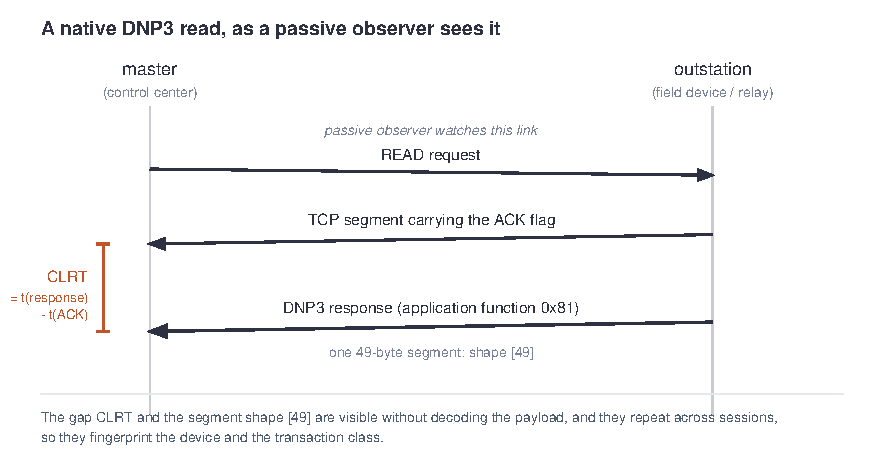
\includegraphics[width=0.98\columnwidth]{figures/fig_native}
\caption{A native read as a passive observer sees it. After the request, the outstation sends a TCP
segment carrying the ACK flag and then the DNP3 application response (function~0x81). The cross-layer
response time (CLRT) is the interval between those two packets; the response is a single 49-byte
segment, a shape we write $[49]$.}
\label{fig:native}
\end{figure}

\subsection{The native control transaction}
Control is a two-step exchange called select-before-operate. The master first sends a SELECT that
arms a control point; the outstation confirms it. The master then sends an OPERATE that actuates the
point, and the outstation echoes the command back. The two steps exist so that a stray or replayed
OPERATE with no matching SELECT cannot act.

\subsection{The observation point}
We assume a passive observer on the \emph{master-facing} link, the segment between the master and the
switch. It records TCP and IP headers, TCP segment sizes, and arrival times. It does not see the
\emph{relay-facing} link between the switch and the outstation, nor anything internal to the switch.
Fig.~\ref{fig:threat} places the observer and marks the relay-facing link as unobserved.

\begin{figure}[t]
\centering
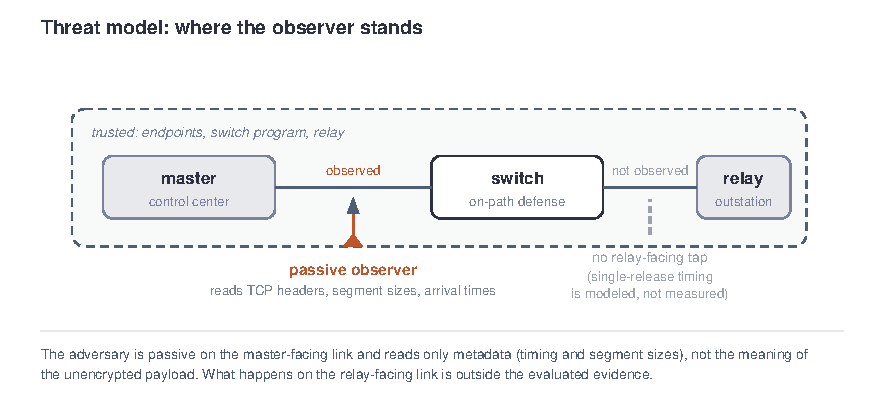
\includegraphics[width=0.98\columnwidth]{figures/fig_threat}
\caption{Threat model. The passive observer sits on the master-facing link and reads only metadata
(TCP headers, segment sizes, arrival times). The relay-facing link is not observed, so the internal
release timing of a control command is modeled, not measured.}
\label{fig:threat}
\end{figure}

\subsection{The two leaked features}
From that vantage the observer reads two features without decoding the payload. The \emph{cross-layer
response time} is the gap between the ACK-bearing segment and the DNP3 response defined above; it
reflects the outstation's internal processing. The \emph{segment shape} is the vector of TCP segment
sizes the response is delivered in ($[49]$ natively). Because the outstation is deterministic, both
features repeat across sessions, so they fingerprint the device and separate its transaction classes:
on the SEL-751 the read and select classes differ in CLRT (medians near 1.3 and 2.1~ms).

\subsection{What defended traffic should look like}
The defense produces two changes on the master-facing link, shown in Fig.~\ref{fig:shape}. It fixes
the CLRT to a single policy value, so the timing no longer separates the classes. And it fixes the
segment shape to $[28,21]$: the same 49 bytes, now delivered as two segments of 28 and 21 bytes. The
cut is placed at a boundary DNP3 already uses. A DNP3 frame is a link header followed by 16-byte data
blocks, each closed by a 2-byte CRC that the master validates; cutting between two such blocks yields
two segments that each end on an already-valid CRC, so no byte is edited and no CRC is recomputed.
Byte~28 is one such boundary. The reassembled response is still 49 bytes: the defense normalizes the
observed shape and timing, not the total length, which a full TCP reader still recovers.

\begin{figure}[t]
\centering
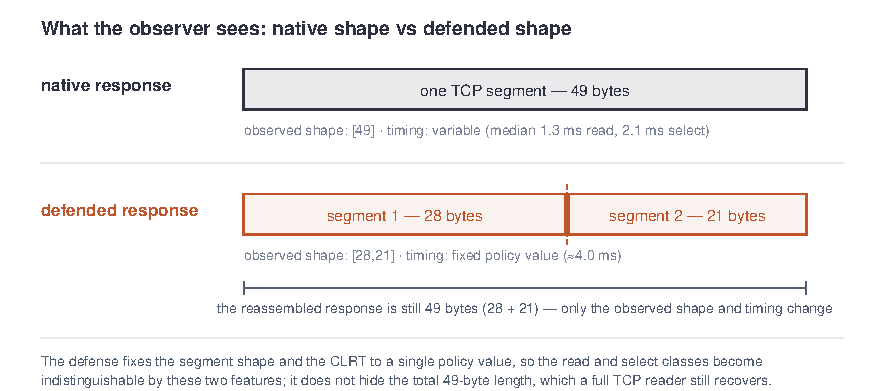
\includegraphics[width=0.98\columnwidth]{figures/fig_shape}
\caption{Native versus defended, as observed. The native response is one 49-byte segment with variable
timing; the defended response is the same 49 bytes as a fixed $[28,21]$ two-segment shape with a fixed
CLRT. The total length is unchanged.}
\label{fig:shape}
\end{figure}

\subsection{The two treatments and why they are separated}
Two treatments produce these changes. \emph{Response shaping} handles a read or select response: it
holds the acknowledgment and the response, releases each at a fixed offset from the request so the
CLRT is a constant, and splits the released response into the $[28,21]$ shape. \emph{The
control-command treatment} handles the OPERATE: it holds the command and releases it once at an
internal delay, while pinning the master-visible acknowledgment and echo to the request's arrival so
that the observable gap does not vary with the internal delay. The two treatments cannot share one
priority schedule. Response shaping keeps a set of higher-priority ``blocker'' packets draining to
time its release; if the held control command sat below them on the same schedule, those blockers
would starve it and its release would drift toward the response's release time instead of its own.
The design therefore gives the two treatments \emph{two independent scheduling lanes} inside the same
switch, as Fig.~\ref{fig:scheduler} shows; both are internal paths in one switch and one program, not
extra devices or a second pipeline.

\section{Threat Model, Assumptions, and Goals}
\label{sec:threat}

\subsection{System and adversary}
The system is the master, the switch, and the SEL-751 outstation of Section~\ref{sec:bg}, exchanging
the native read and control transactions defined there. The adversary is a \emph{passive} observer on
the master-facing link: it captures traffic from a mirrored port or a tap and does not modify, inject,
or block a packet. Its goal is reconnaissance, to fingerprint the outstation and its transactions from
what the traffic exposes.

\subsection{What the adversary can and cannot read}
The adversary reads metadata: TCP and IP headers, TCP segment sizes, and arrival times. The traffic is
unencrypted, so the DNP3 payload is in fact parseable; our threat, however, uses only the two
metadata features of Section~\ref{sec:bg} (CLRT and segment shape) and does not depend on application
semantics. Following Formby et~al.~\cite{formby2016}, we distinguish three fingerprinting aims: device
identity, device type, and transaction-class inference. Our evaluation concerns transaction-class
inference (separating read from select by CLRT) on one device, and the replacement of that device's
evaluated features; we do not claim device-identity results or indistinguishability among devices. The
adversary knows the protocol and may know the defense policy; its advantage comes only from observing
the features.

\subsection{Trusted computing base and deployment assumptions}
The master, the switch and its loaded program, and the outstation are trusted. The defense runs
entirely in the switch data plane, with no host agent, controller fast path, or endpoint change. Two
deployment assumptions bound the timing argument. First, the protected flow carries no TCP timestamp
option, which would be an independent timing channel; in our evaluation the option was disabled on the
host and confirmed absent at the packet level in a preflight check, and the switch program also parses
the option so the timing argument is asserted only when it is absent. Second, only the eligible
response class (here the 49-byte read and control responses) is shaped; other traffic is forwarded
unchanged.

\subsection{Security goals}
We state the security goals as testable properties of the master-facing observation. \textbf{G1:} the
defended CLRT is a single policy value independent of the transaction class. \textbf{G2:} every
eligible response presents the fixed segment shape $[28,21]$. \textbf{G3:} the master reassembles a
sequence-contiguous, CRC-valid, checksum-valid 49-byte response. \textbf{G4:} for a control command,
the master-visible acknowledgment and echo placement does not vary with the internal release delay.
\textbf{G5 (safety):} the defense actuates no physical output. A separate evaluation-validity
property, that native and defended traffic differ only by a runtime mode on one loaded program, lets
the comparison isolate the defense; we treat it as a methodology control rather than a security goal.

\subsection{Non-goals and evidence limitations}
The following are out of scope, and the evidence does not establish them. We do not verify the
relay-facing link: the internal release time and the number of copies delivered to the relay are not
captured, so the single release is a modeled, not a measured, property, and we do not claim
exactly-once delivery. We do not hide the total response length, which stays 49 bytes and is
recoverable by a full TCP reader. We do not claim byte identity between an emitted response and a
source frame, because no paired source-side oracle was captured. We do not generalize from one
SEL-751 and one eligible class to all DNP3 outstations, and we do not claim indistinguishability among
devices or resistance to every traffic-analysis feature. We do not defend against an active adversary
or add payload confidentiality. If the observer could also see the relay-facing link, it could time
the internal release directly, and the control-command timing property would no longer hold; the
defense is scoped to the master-facing observer.

\section{Implementation}
\label{sec:impl}

We implement the design of Section~\ref{sec:bg} as one P4 program on a single Intel Tofino-1 switch,
with a control-plane configuration layer and a guarded control-test harness. This section starts with
an end-to-end walkthrough, then details each mechanism. For each mechanism we give the same account:
the problem it solves, the packet or state that triggers it, the observable effect, the failure
behavior, and the evidence that verifies it. Switch-internal names (ports, queues, tables) appear only
after the concept they implement.

\subsection{End-to-end walkthrough}
A read enters the switch from the master. The program records the request's arrival time, forwards the
request to the relay, and prepares to hold the relay's answer. When the acknowledgment and the
response come back, the program holds each in a switch queue and releases them at fixed offsets from
the recorded request time, so the master sees a constant CLRT; on release it replicates the response
and emits it as the two segments $[28,21]$. A control command is handled on a second internal path:
the SELECT prepares a hold, the OPERATE is admitted once and held, and it is released to the relay at
an internal delay, while the acknowledgment and echo the master sees are placed at fixed offsets from
the OPERATE's arrival. Two internal scheduling lanes keep the response path and the command path from
interfering. A single terminal decision applies every forwarding effect.

\subsection{Physical topology and packet paths}
The master reaches the switch on one port and the switch reaches the SEL-751 on another; these are the
only external cables. Three further ports are internal to the switch and carry no cable: two
recirculation paths give the response treatment and the control treatment their own scheduling lanes,
and one path is used by the switch's packet generator. The adversary observes only the master-facing
port; the relay-facing port and the internal paths are not observed. Fig.~\ref{fig:pipeline} shows the
detailed topology and names the internal ports and queues.

\begin{figure*}[t]
\centering
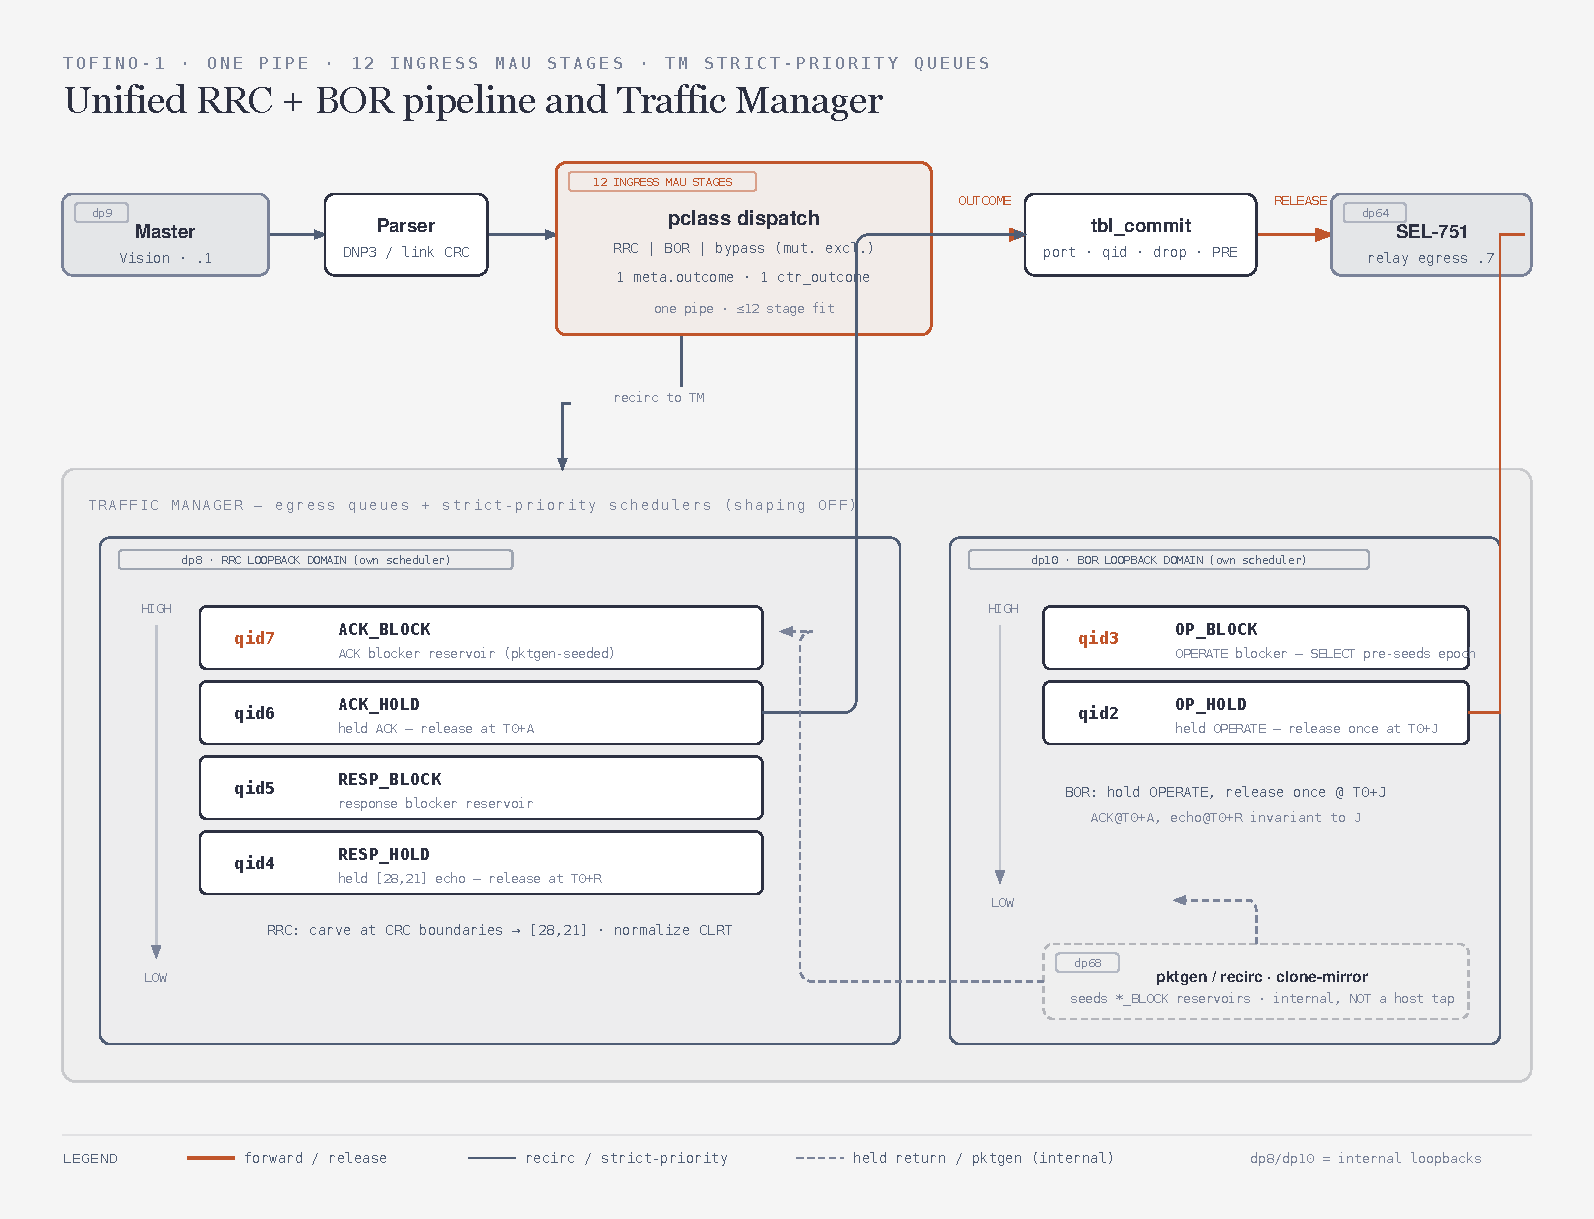
\includegraphics[width=0.95\textwidth]{figures/fig_pipeline}
\caption{Detailed switch pipeline. The parser and match-action stages compute one compact outcome that
a single terminal table applies; the Traffic Manager holds the response reservoirs and queues on one
internal lane (\code{dp8}) and the control queues on a second (\code{dp10}), with the packet generator
(\code{dp68}) seeding the reservoirs; egress carves the eligible response to $[28,21]$. Port and queue
names appear only here.}
\label{fig:pipeline}
\end{figure*}

\subsection{Recording the request time and arming deadlines}
\textbf{Problem.} A held packet must be released at a fixed offset from the request, but the switch has
no general-purpose timer. \textbf{Mechanism.} On the request (or the OPERATE), the program records an
ingress timestamp $T_0$ and arms two deadlines, $T_0{+}A$ for the acknowledgment and $T_0{+}R$ for the
response, from the policy offsets $A$ and $R$; the master-visible CLRT is then $R-A$. Anchoring to
$T_0$ rather than to the relay's later acknowledgment matters for the control command: because that
acknowledgment exists only after the held OPERATE is released, anchoring to it would leak the hold. An
offline model checks this anchoring against a mutant that arms the deadline at the acknowledgment, and
the mutant is killed.

\subsection{Reservoirs as data-plane timers}
\textbf{Problem.} Realize a deadline from packet scheduling alone. \textbf{Mechanism.} A held packet
waits in its queue behind a higher-priority reservoir of small ``blocker'' packets; a strict-priority
scheduler drains the blockers first, so the held packet cannot leave until its reservoir empties,
which the control plane sizes to the policy deadline. The switch's on-chip packet generator fills the
reservoirs and never generates master or relay traffic. Two generator profiles are distinguished by a
tag byte so that a read or select arm and a control hold trigger different reservoirs without
ambiguity.

\subsection{Response shaping: hold, release, replicate, carve}
Response shaping normalizes the timing and shape of an eligible 49-byte response. The acknowledgment
and the response are held in strict-priority queues and released at $T_0{+}A$ and $T_0{+}R$. On
release the program steers the response into the switch's packet-replication engine, which produces
two master-facing copies; egress then emits the 28-byte prefix from one copy and the 21-byte suffix
from the other, advancing the suffix's TCP sequence number by 28 so the two segments abut. The relay
produces the response; replication produces the two copies used for segmentation, and no clone
fabricates the response. By design the program edits no DNP3 byte and recomputes no DNP3 CRC, updating
only the IP and TCP checksums per segment; the hardware evidence bounds this to a sequence-contiguous,
CRC-valid, checksum-valid 49-byte reconstruction, not byte identity to a source frame. The 49-byte
frame is a 10-byte link header, an 18-byte first data block (16 data + 2 CRC), a second 18-byte block,
and a 3-byte final block; byte~28 falls between the first and second blocks (Fig.~\ref{fig:carve}).
TCP may segment a byte stream at any offset, so cutting at byte~28 is a design and verification
choice that keeps each segment aligned to a completed CRC block, not a TCP requirement.

\begin{figure}[t]
\centering
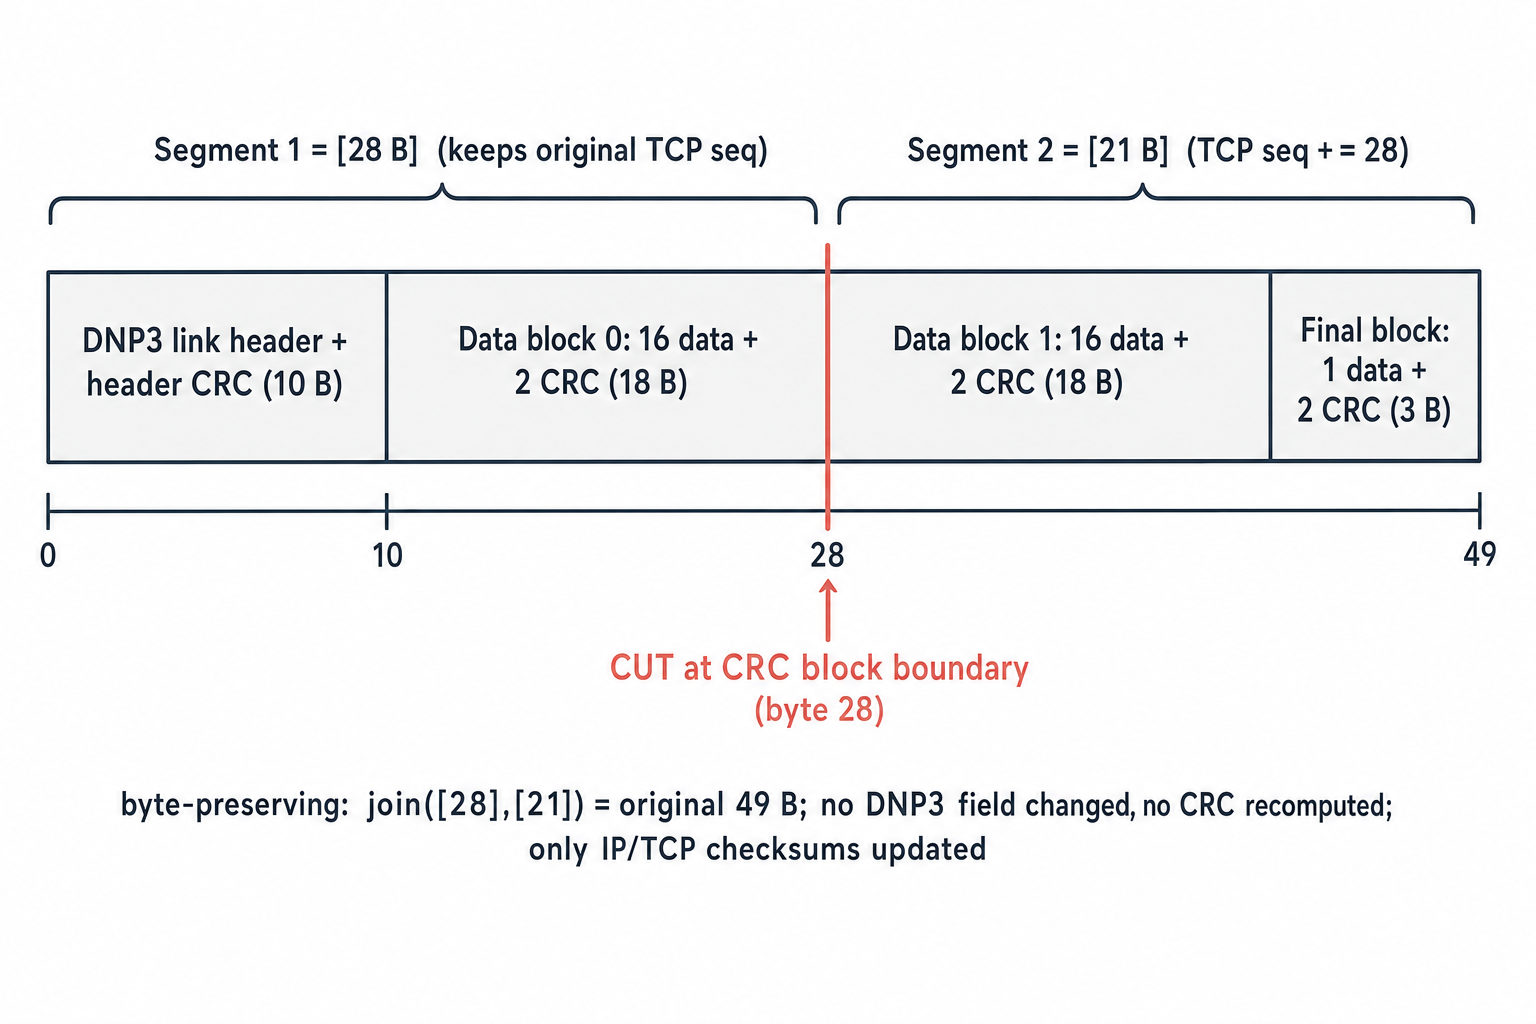
\includegraphics[width=0.98\columnwidth]{figures/fig_carve}
\caption{The 49-byte response and the $[28,21]$ carve. The cut at byte~28 is a boundary DNP3 already
places between CRC-protected blocks; the prefix keeps the original TCP sequence number and the suffix
advances it by 28. No DNP3 byte is edited and no DNP3 CRC is recomputed.}
\label{fig:carve}
\end{figure}

\subsection{The control command and its state}
\textbf{Problem.} An outbound OPERATE exposes an operation-timing fingerprint, and releasing it on a
fixed schedule would still reveal it. \textbf{Mechanism.} The SELECT prepares a hold by seeding the
control reservoir, so the hold is armed before the OPERATE arrives. The switch admits one matching
OPERATE, holds it, and releases it once to the relay at an internal delay drawn in the data plane from
a bounded set. The master-visible acknowledgment and echo are released at $T_0{+}A$ and $T_0{+}R$,
anchored to the OPERATE's own arrival and independent of the internal delay, so the observable gap
carries no information about it. After release the transaction's generation is kept as a spent marker
until the next SELECT; a retransmitted OPERATE that reads the spent marker is treated as a duplicate
and dropped. \textbf{Evidence boundary.} The hardware captures establish the master-visible placement
and the delay-invariant gap; the offline model verifies the single release; the relay-facing release
time and the number of copies delivered are not captured, so single release is modeled, not measured.

\subsection{Two independent scheduling lanes}
Response shaping seeds acknowledgment and response reservoirs on high-priority queues. On one shared
strict-priority schedule these reservoirs starve the control hold that would sit below them, shifting
its release toward the response's release time instead of its own deadline
(Fig.~\ref{fig:scheduler}a). The design places the response queues on one internal recirculation lane
and the control queues on a second (Fig.~\ref{fig:scheduler}b), so each arbitrates on its own
scheduler. A register-domain separation keeps a control-path packet from touching the response path's
state. Both lanes are internal to the same switch and the same program.

\begin{figure}[t]
\centering
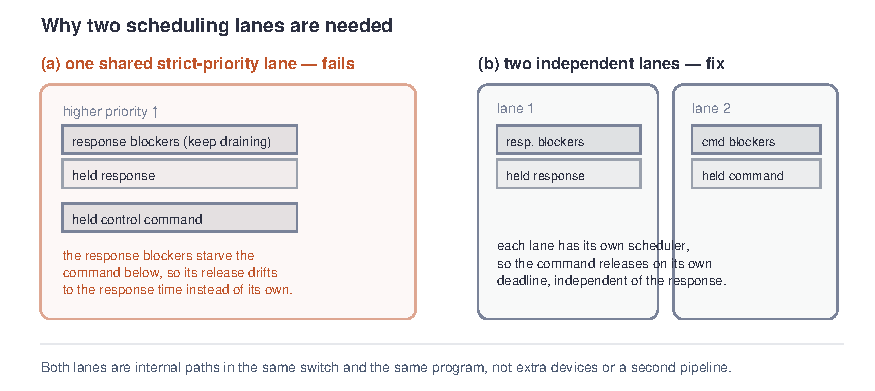
\includegraphics[width=0.98\columnwidth]{figures/fig_scheduler}
\caption{Why two scheduling lanes are needed. (a) On one shared strict-priority schedule, the
response's blocker packets starve the held control command below them, so its release drifts to the
response's release time. (b) Two independent lanes each carry their own blockers and held packet, so
the command releases on its own deadline. Both lanes are internal to the same switch and program.}
\label{fig:scheduler}
\end{figure}

\subsection{One outcome, one commit}
Earlier match-action stages compute one compact result and a single terminal table applies it. The
terminal table is keyed on that result and is the only stage that sets the egress port, the queue, a
drop, a bypass, or a multicast group; every defined result is mapped by a constant entry. The default
action, taken only for the otherwise-unreachable unset result, forwards the packet unmodified rather
than dropping it. This is distinct from the explicit dispositions of recognized traffic: internal-only
packets such as a bad-port packet, a returning generator token, a clone, a duplicate response, or a
retired blocker are mapped to an explicit drop, while a recognized but ineligible or unsupported
response is mapped to an explicit forward. The single-table structure keeps the disposition auditable
and, with a flattening of the decision logic into two mutually exclusive tables that co-place in one
stage, lets the whole program fit one ingress pipeline within its stage budget.

\subsection{Control plane, failure behavior, and safety}
The control-plane layer brings up the ports, creates the queues at descending strict-priority levels
with shaping disabled, installs the multicast group and the generator profiles, writes the timing
parameters and the internal-delay set, and initializes the state. Every write is read back and
compared, and a mismatch or a configuration warning leaves the mechanism disabled rather than
partially configured; there is no configuration snapshot, and rollback is a forward, readback-checked
teardown to a plain forwarding state. Traffic outside the eligible class, unsupported functions, and
malformed frames are forwarded unchanged. The control-test harness that issues a physical SELECT and
OPERATE is guarded: it permits only two isolated control points and refuses a breaker-close point.
Across every guarded transaction all 32 relay outputs remained open and no breaker operation was
attempted.

\subsection{Resource fit and limitations}
The program compiles for one Tofino-1 ingress pipeline within the twelve-stage match-action budget.
The evaluation is on physical hardware, one switch and one relay; it is not a deployment study. The
implementation does not observe the relay-facing link, does not normalize total response length, and
is evaluated on one outstation and one eligible response class; Section~\ref{sec:eval} reports the
measured consequences of these bounds. The loaded source and binary are identified by hash, the
analysis regenerates deterministically from the captured traces, and a manifest verifies every derived
artifact.

\section{Evaluation}
\label{sec:eval}

We evaluate on a testbed with a physical master, one Tofino-1 switch, and a physical SEL-751 relay.
Native and defended traffic are captured on the same loaded program, separated only by a runtime mode
change, so the comparison isolates the defense. The defended captures carry no TCP timestamp option.
The analysis regenerates deterministically from the traces, and a manifest verifies every derived
artifact. Throughout, we separate what the hardware captures measure on the master-facing link from
what the offline model verifies and what is not observed.

\noindent\textbf{Timing (measured).} The native CLRT median is 1.272~ms for read (standard deviation
1.354, $n{=}999$) and 2.107~ms for select ($n{=}488$), with heavy tails. The defended CLRT median is
4.001~ms for both classes, with standard deviation 0.022 and 0.021~ms, matching the policy $R-A=4$~ms.
The master-facing offsets $A$ and $R$ measure about 21 and 25~ms, which include a documented path and
capture offset of roughly 1~ms over the configured 20 and 24~ms; the internal switch deadline was not
instrumented separately.

\noindent\textbf{Shape and reconstruction (measured).} The native read is one 49-byte segment. All
1{,}280 defended eligible responses (600 read, 500 select, and 90 select with 90 operate from the
control transactions) present the $[28,21]$ shape. Each is sequence-contiguous, valid under the DNP3
link and block CRCs, and valid under the IP and TCP checksums, and no defended response escapes as an
unsplit 49-byte segment. Because no paired source-side capture exists, we report a CRC- and
checksum-valid reconstruction, not byte identity to a source frame.

\noindent\textbf{Control-command timing (measured and modeled).} Fig.~\ref{fig:timeline} shows the
master-facing acknowledgment and echo of a control command. The echo-minus-acknowledgment gap is
4.00~ms and does not vary with the internal release delay: across the evaluated delays of 2, 6, and
12~ms the pooled gap median is 4.002~ms with standard deviation 0.026~ms ($n{=}90$). The relay-facing
release time and the number of copies delivered to the relay are not captured; the offline model
verifies the single release, and the captures establish that the master issued one OPERATE per
transaction.

\begin{figure}[t]
\centering
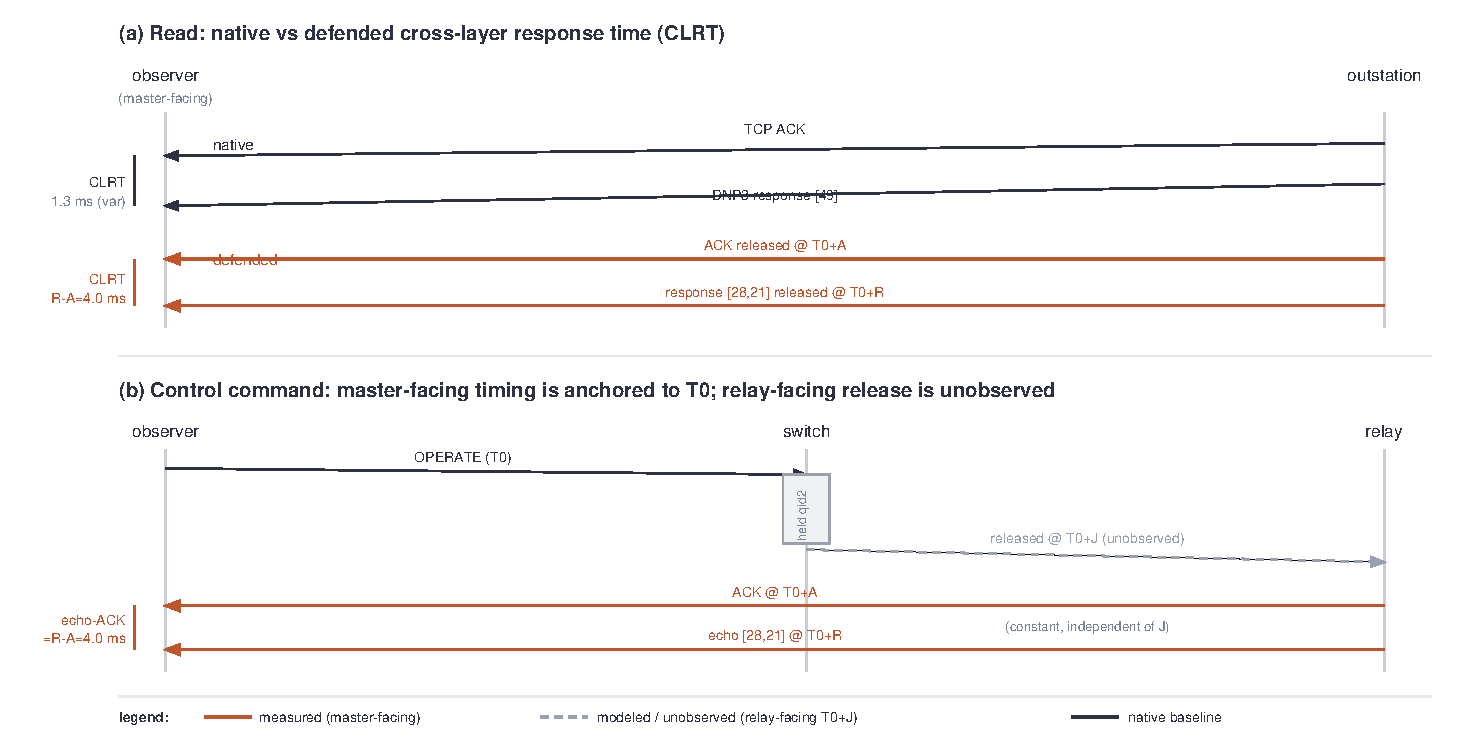
\includegraphics[width=0.98\columnwidth]{figures/fig_timeline}
\caption{Native versus defended timing, and the control-command timeline. The defended acknowledgment
and response are placed at $T_0{+}A$ and $T_0{+}R$; the internal release at $T_0{+}J$ is on the
relay-facing link and is not captured (dashed), so it is verified by the model rather than measured.}
\label{fig:timeline}
\end{figure}

\noindent\textbf{Fingerprint suppression (measured).} We quantify the leak with the mutual information
between the transaction class and the CLRT, using common bins and a permutation null. The native
mutual information is 0.424~bits, well above the null band, and the defended value is 0.0018~bits,
inside it. A logistic classifier trained to separate read from select by CLRT reaches 0.592 balanced
accuracy on native traffic and 0.500, the chance baseline, on defended traffic. This is a
transaction-class task on one device, not a device-identity task; the defense replaces the evaluated
CLRT and segment-shape features of this SEL-751 and does not establish indistinguishability among
devices.

\noindent\textbf{Safety and resource fit (measured).} The guarded control test permitted only two
isolated control points and refused the breaker-close point; all 32 relay outputs remained open
throughout, and no breaker operation was attempted. The program compiles for one ingress pipeline
within the twelve-stage budget.

\section{Discussion}
\label{sec:disc}

The defense replaces two master-facing features of one outstation with a fixed policy while preserving
the protocol. It does not hide the total 49-byte length, which a full TCP reader recovers, and it does
not establish indistinguishability among devices or resistance to every traffic-analysis feature.
Extending the eligible class beyond the 49-byte responses would require a segment-shape policy for each
response size; the CRC-block structure supports this, but we have not evaluated it. The strongest open
item is relay-facing verification: a tap on the relay-facing link would turn the modeled single
release into a measured property, and we leave that instrumentation to future work.

\section{Related Work}
\label{sec:related}

\noindent\textbf{Device fingerprinting.} Devices are identifiable from wire-side behavior without
payload access: from remote clock skew~\cite{kohno2005}, from timing signatures that reveal device and
device type~\cite{gtid2015}, and, for cyber-physical systems, from cross-layer response timing,
physical-operation timing, and device physics~\cite{formby2016,gu2018}. This line defines the threat
we address rather than a defense. Our objective differs: we suppress the master-facing CLRT and
segment-shape features these techniques exploit, for one evaluated device and its transaction classes.

\noindent\textbf{Network-timing traffic analysis and its defenses.} Inter-event timing leaks content,
from keystroke intervals on SSH~\cite{song2001} to timing-only web-page recovery~\cite{feghhi2016} and
deep-learning website fingerprinting~\cite{sirinam2018}, though such accuracy is contested at realistic
open-world scale~\cite{panchenko2016}. Defenses shape the traffic: adaptive padding breaks the
inter-packet pattern~\cite{juarez2016}, comprehensive side-channel mitigation shapes a tenant's
traffic to a leak-free schedule~\cite{pacer2022}, and anonymity systems resist traffic analysis at the
network layer~\cite{hornet2015,taranet2018}. These target browser or cloud traffic and assume a
cooperating end host or hypervisor that can add cover traffic. Our defense normalizes the
acknowledgment-to-response timing of a protocol-bound DNP3 exchange in the network, with no endpoint
change and no added application bytes, and fixes one cross-layer interval rather than obscuring a
distribution.

\noindent\textbf{Packet-size padding, morphing, and constant-rate shaping.} Size defenses reshape a
flow's length signature: morphing transforms one class's distribution into another's~\cite{wright2009},
dependent link padding bounds low-latency leakage~\cite{wang2008dlp}, and constant-rate and
burst-molding schemes fix the rate at a cost that is acceptable for one flow but prohibitive across a
device fleet~\cite{tamaraw2014,walkietalkie2017}; later analysis shows per-packet padding and
fragmentation still leave exploitable features~\cite{dyer2012}. The same size-and-rate channel
identifies devices even under encryption, where shaping, made differentially private, is the
countermeasure~\cite{apthorpe2019,netshaper2024}. These change or pad bytes and target the end host.
Our mechanism neither pads nor rewrites DNP3 bytes; it re-segments the response only at existing
CRC-block boundaries, so the reassembled message and every per-block CRC are preserved while the
observed shape is fixed.

\noindent\textbf{Reconnaissance, moving-target defense, and DNP3 security.} A body of work disrupts
grid reconnaissance rather than detecting its use: DefRec virtualizes physical functions to present
deceptive content and connectivity~\cite{defrec2020}, RAINCOAT randomizes data acquisition and injects
decoys~\cite{raincoat2019}, and a companion testbed evaluates such approaches on grid cyber-physical
infrastructure~\cite{lintestbed2020}; the reconnaissance these blunt ultimately enables
false-data-injection and process-control attacks~\cite{liufdia2009,cardenas2011,sridhar2012}. A
parallel line detects rather than obfuscates, adapting specification-based and state-based intrusion
detection to DNP3 and analyzing its attack surface~\cite{linbro2013,fovino2010,east2009}, and in-network
obfuscation has denied reconnaissance by rewriting data-plane topology against link-flooding
attacks~\cite{nethide2018}. These operate at the content, connectivity, topology, or detection layer.
Our defense instead obfuscates the wire-visible timing and shape of the transport exchange itself,
below the semantics those defenses reshape, and complements rather than replaces them. Standards and
incident analyses frame the setting~\cite{dnp3std,ukraine2015,nist80082}.

\noindent\textbf{Timing and shaping on programmable switches.} Programmable data planes make in-network
shaping practical. The P4 model exposes a programmable parser and match-action
pipeline~\cite{p4ccr2014}; push-in-first-out queues define ideal programmable
scheduling~\cite{pifo2016}, and SP-PIFO approximates it with a few strict-priority queues on today's
switches~\cite{sppifo2020}, the primitive class our deadline scheduler uses. Recent systems bring
traffic-analysis defense fully into the data plane: Ditto pads and injects chaff to a fixed WAN
pattern~\cite{ditto2022}, Securitas obfuscates flows with flexible in-network
shaping~\cite{securitas2026}, Minos mounts a dynamic defense on programmable switches~\cite{minos2025},
and, closest to our setting, Hu and Lin enhance industrial-protocol security with programmable
switches~\cite{hulin2023}. Our defense differs from these in two ways: it is byte-preserving and carves
only at existing DNP3 boundaries, so the outstation's protocol remains valid, and it adds a
control-command treatment that hides operation timing from the master-facing observer without exposing
the hold.

\section{Conclusion}
\label{sec:concl}

An observer of unencrypted DNP3 traffic can fingerprint an outstation from the cross-layer response
time and the segment shape of its responses, and neither encryption, endpoint changes, nor generic
traffic-analysis defenses fit the constraints of a deployed DNP3 link. We placed the defense in the
data plane of one programmable switch, where it holds the acknowledgment and response and releases them
at fixed offsets from the request to normalize the response time, replicates and carves the eligible
response into a fixed $[28,21]$ shape at an existing CRC boundary, and holds a control command to pin
its master-visible timing to the request. On a physical SEL-751 relay the defended cross-layer response
time is a fixed 4.001~ms, every eligible response presents the $[28,21]$ shape with a CRC- and
checksum-valid reconstruction, the control-command gap stays at 4.00~ms across the evaluated internal
delays, and a read-versus-select timing classifier falls to chance, within a single-device,
master-facing evaluation boundary whose relay-facing verification we leave to future work.


\bibliographystyle{IEEEtran}
\bibliography{rewrite/refs}

\end{document}
